%% The following is a directive for TeXShop to indicate the main file
%!TEX root = ../MJThesis.tex
\acresetall

\chapter{Introduction}
\label{ch:Introduction}

\begin{epigraph}
    \emph{But during the writing of this review, I learned how little I knew in this area, and this was a humbling and sobering experience. I am certain that I have made many mistakes due to my ignorance, and I hope that the review will be useful despite its many faults} ---~Hiroshi Nikaido (2003), my grand supervisor.
\end{epigraph}

\section{History of S-layers} % (fold)
\label{sec:history_of_s_layers}
   

    \begin{figure}[p] % First S-layer
            \begin{center}
                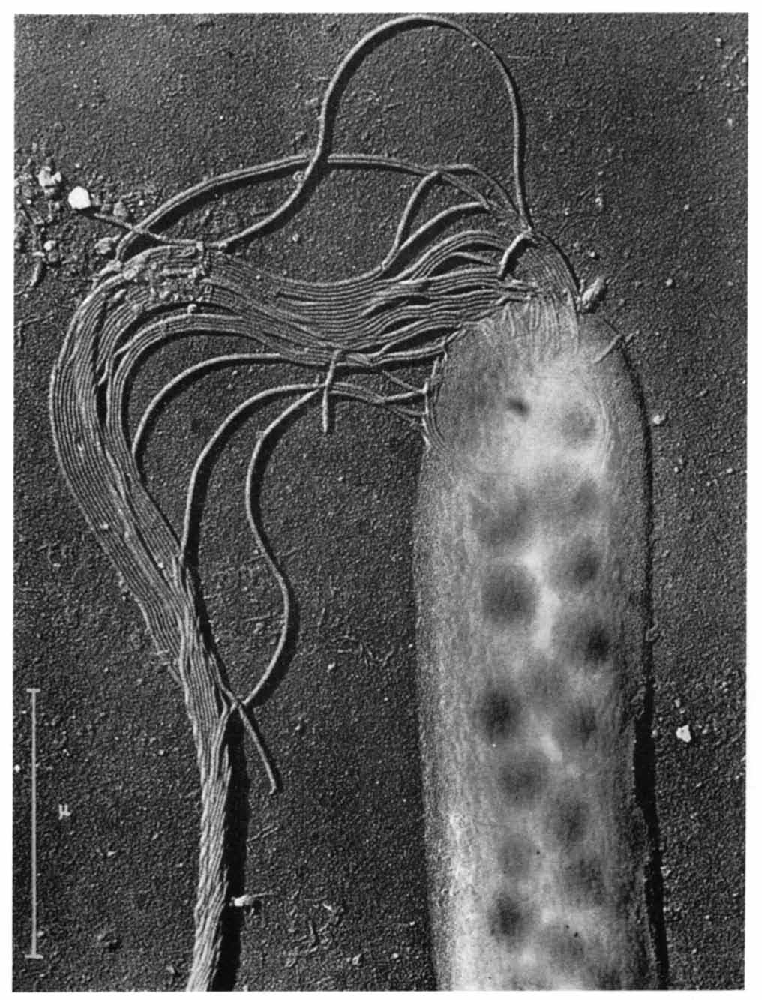
\includegraphics[]{intro/img/firstslayer.pdf}
            \end{center}
            \caption[The first published image of a \ac{S-layer}.]{The first published image of a \ac{S-layer}. The hexagonal \ac{S-layer} on the surface of the bacterium --- probably \textit{Spirillum} sp. --- is visible along the edges of the cell body (centre right). The scale bar denotes one micrometre. (This image is Fig. 1 from \fullcite{firstslayer} )}
            \label{fig:firstslayer}
    \end{figure}
    
    \begin{figure}[p]
        \begin{center}
            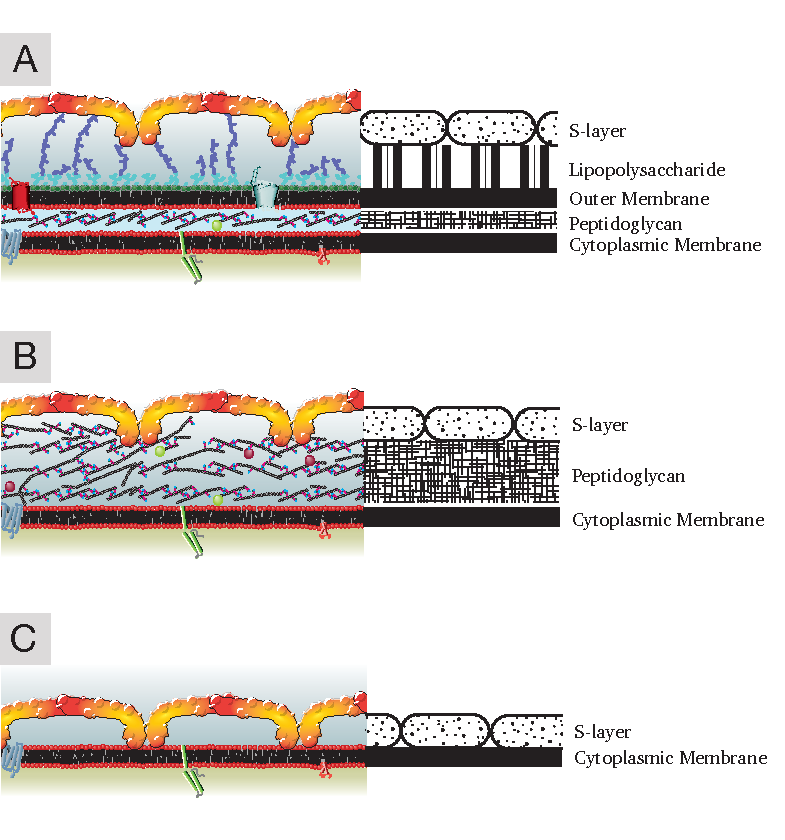
\includegraphics[]{intro/img/celwalls.pdf}
        \end{center}
        \caption[Cross-sectional diagrams of the cell envelopes]{Cross-sectional diagrams of the cell envelopes of (\textbf{A}) Gram negative bacteria, (\textbf{B}) Gram positive bacteria, and (\textbf{C}) archaebacteria. In all known cases the \ac{S-layer} sits on the extreme outer surface of the cell. (This diagram was inspired by Fig. 1 from \fullcite{sleytr1983crystalline})}
        \label{fig:cellwalls}
    \end{figure}
% section history_of_s_layers (end)


\endinput

Any text after an \endinput is ignored.
You could put scraps here or things in progress.
